\part{Part 2: Physics}

\chapterimage{chapter_head_2.pdf} % Chapter heading image

\chapter{Conservation Laws}
Some of the most powerful tools in classical mechanics, including fluid mechanics, are conservation laws. Arising from the profound physical insights of Newton, Leibniz, and others, these laws ensure that the total amount of certain physical quantities within a volume are conserved. For example, conservation of mass ensures that the total mass of a system remains constant, conservation of momentum ensures that the total momentum of a system remains constant, and conservation of energy ensures that the total energy of a system remains constant. That is, given an isolated physical system, the total mass, momentum, and energy should remain constant and, conversely, for an open system the change in mass, momentum, and energy is equal to the amount that enters/leaves the system across its boundaries.

While these concepts can be applied by a high-school student for simple systems, such as elastic/inelastic collisions between partciles, their application to fluid mechanics is less trivial. Nevertheless, the fundamental concepts of conservation of mass, momentum, and energy still apply to fluids just as well as they do to individual particles, it is only the mathematics that becomes more complex. It is expected that students reading this book have already taken an undergraduate course in fluid mechanics and are familiar with conservation laws. Nevertheless, this chapter reviews these concepts for completeness, and to establish the notation used in the rest of the book.

\section{Reynolds Transport Theorem}\index{Reynolds Transport Theorem}
Before tackling conservation of mass, momentum, and energy in their entirety, we will first consider an arbitrary conserved {\it extensive} quantity $U_{System} = U_{System}(t)$ of a moving system of fluid, which has a related quantity per unit volume $u = u(\vec{x},t)$, where $\vec{x}$ and $t$ are the spatial coordinate and time, respectively. For example, if the extensive property is mass, than the volumetric property is mass per unit volume, or density. We start by imagining a stationary control volume (CV), denoted by $\Omega$, that is the same shape as the fluid system at some time $t$. We also denote the surface of this volume by $S$ and the outward pointing normal vector on this surface by $\hat{n}$. After some amount of time $dt$, we can imagine that the initial system of fluid embedded within the control volume will move to a deformed position and shape at $t + dt$, while the control volume remains fixed by definition. In this manner the fluid contained by the system will be equal to that of the control volume plus any incoming or outgoing fluid due to the motion of the system system boundaries as it travels with the flow.

Looking at Figure \ref{}, there are two ways that $U_{System}$ will change with time. Either via a change of $U_{CV}$ within the control volume it overlaps with, or by some amount of the conserved quantity crossing the boundary of the system as it moves. We start by getting the total amount within the control volume $U_{CV}(t)$ by simply adding up, or integrating, $u$ over it. This can be written as
\begin{equation}
	\label{eqn:totalcons}
	U_{CV}(t) = \int_\Omega u d\vec{x},
\end{equation}
noticing that the dependence on space is lost after integration. The time derivative of this is associated with the rate of change of the conserved variable within the control volume itself
\begin{equation}
	\label{eqn:totalcons}
	\frac{dU_{CV}}{dt} = \frac{d}{dt}\int_\Omega u d\vec{x}.
\end{equation}
The second term to be addressed is the change in $U_{System}$ due to its moving boundaries.

As noted previously, the second way for $U_{System}$ to change with time is by fluid crossing the surface $S$ as the fluid system moves to $t+dt$. In order for fluid to cross the surface it must be moving {\it normal} to it, otherwise it will just move along the surface and not enter the control volume. Hence, we can get the velocity component normal to the surface at any point via the normal vector. Then we can get the total amount of $u$ crossing the surface $S$ by adding up, or integrating, the normal flux at every point on the surface
\begin{equation}
	\label{eqn:totalflux}
	F(t) = \oint_S u (\vec{v} \cdot \hat{n}) ds,
\end{equation}
where $F = F(t)$ is the total rate the conserved quantity $U$ enters/leaves the control volume across the surface.

To create our conservation law we combine the concepts in Equations \ref{eqn:totalcons} and \ref{eqn:totalflux}. We note that the rate of change of the total amount of the conserved variable within the system $U_{System}$ is equal to the rate at which the conserved variable changes within the control volume and the rate it enters/leaves across the surface of the system as it moves. Mathematically this can be written as
\begin{equation}
	\frac{dU_{System}}{dt} = \frac{d}{dt}\int_\Omega u d\vec{x} + \oint_S u (\vec{v} \cdot \hat{n}) ds,
\end{equation}
noting that the positive in front of the surface term is due to our normal vector being outward pointing. Known as Reynolds Transport Theorem, this will be the foundation for deriving our conservation of mass, momentum, and energy equations for fluid flows.

\chapter{The Navier Stokes Equations}

\section{Integral Form}\index{Integral Form}
\subsection{Conservation of Mass}
When considering the mass $m = m(t)$ of our system, the mass per unit volume is the density, denoted by $\rho = \rho(\vec{x},t)$. Since the boundaries of our system move with the fluid flow, no mass can enter or leave. Hence, any mass initially within the system is confined therein and the time rate of change of $m$ is zero. Hence,
\begin{equation}
	\frac{dm}{dt} = \frac{d}{dt}\int_\Omega \rho d\vec{x} + \oint_S \rho \vec{v} \cdot \hat{n} ds = 0,
\end{equation}
and conservation of mass can be written as
\begin{eqBox}
\begin{equation}
	\frac{d}{dt}\int_\Omega \rho d\vec{x} + \oint_S \rho \vec{v} \cdot \hat{n} ds = 0.
\end{equation}
\end{eqBox}

\subsection{Conservation of Momentum}
From Newton's second-law we know that the time rate of change of the total momentum of the system is equal to the sum of all forces acting on it. Hence
\begin{equation}
	\sum \vec{F} = \frac{d(m \vec{v})}{dt},
\end{equation}
where the product $m \vec{v}$ is the total momentum of the system. Noting that the momentum per unit volume is $\rho \vec{v}$, and using Reynolds transport theorem we obtain
\begin{equation}
	 \frac{d}{dt}\int_\Omega \rho \vec{v} d\vec{x} + \oint_S \rho \vec{v} (\vec{v} \cdot \hat{n}) ds = \sum \vec{F},
\end{equation}
which requires knowledge of the forces that will act on the system at any given time, which can be split into surface and body terms. In the current context, only surface terms are considered and body terms, such as gravitational forces, are neglected.

The first of the surface forces is due to the pressure surrounding the system. Since pressure acts normal to a surface, the total pressure force $\vec{F_P}$ can be obtained via integration along the surface. Hence,
\begin{equation}
	\vec{F_P} = \oint_S -p\hat{n} ds,
\end{equation}
where $p$ is the pressure and the negative is included since pressure exerts a force inwards, but our normal vector is defined as outwards. The second set of surface terms is due to the effects of viscosity. To account for these we introduce the Cauchy stress tensor $\tau$, which for Newtonian fluids is
\begin{equation}
	\label{eqn:cauchytensor}
	\tau = \mu \left(\nabla \vec{v} + \left(\nabla \vec{v} \right)^T \right) - \frac{2}{3} \mu \left(\nabla \cdot \vec{v} \right) \mathbf{I},
\end{equation}
where $\mu$ is the dynamic viscosity and $\mathbf{I}$ is an identity matrix. Whereas pressure acts normal to the control volume surface, viscous effects act parallel to it. Hence, the total viscous force $\vec{F_v}$ can be obtained via integration
\begin{equation}
	\vec{F_v} = \oint_S \tau \cdot \hat{n} ds.
\end{equation}
With the inviscid and forces determined, conservation of momentum can be written as
\begin{equation}
	 \frac{d}{dt}\int_\Omega \rho \vec{v} d\vec{x} + \oint_S \rho \vec{v} (\vec{v} \cdot \hat{n}) ds = \oint_S -P\hat{n} ds + \oint_S \tau \cdot \hat{n} ds,
\end{equation}
which is commonly written by grouping all of the surface integral terms
\begin{eqBox}
\begin{equation}
	 \frac{d}{dt}\int_\Omega \rho \vec{v} d\vec{x} + \oint_S \left[ \rho \vec{v} \oplus \vec{v} - \sigma \right]\cdot \hat{n} ds =  0,
\end{equation}
\end{eqBox}
where
\begin{equation}
	\sigma = -p \mathbf{I} + \tau.
\end{equation}

\subsection{Conservation of Energy}
From conservation of energy, the rate of change of energy within the system is equal to the rate of heat added to the system less the rate work done by the system on its surroundings. Hence,
\begin{equation}
	\frac{dE}{dT} = \frac{dQ}{dT} - \frac{dW}{dT},
\end{equation}
where $E$ is the energy in the system, $Q$ is heat, and $W$ is work. In this case the energy per unit volume is $\rho e$ where 
\begin{equation}
e = c_v T + \frac{1}{2} \vec{v} \cdot \vec{v},
\end{equation} 
is the specific energy, $c_v$ is the specific heat at constant volume, and $T$ is the temperature. Using Reynolds transport theorem we have
\begin{equation}
\frac{d}{dt}\int_\Omega \rho e d\vec{x} + \oint_S \rho e (\vec{v} \cdot \hat{n}) ds = \frac{dQ}{dT} - \frac{dW}{dT}.
\end{equation}

Since body forces have been neglected, the work done by the system on its surroundings is due to only surface forces. The work done by pressure $\dot{W}_p$ is due to the product of the pressure force, which acts normal to the boundary, and the velocity of the boundary in the normal direction. Hence,
\begin{equation}
	\dot{W}_p = \oint_S p(\vec{v} \cdot \hat{n}) ds.
\end{equation}
Similarly, the work done by viscous forces, $\dot{W}_v$, is due to the product of the viscous stresses and the velocity on the surface. Hence, 
\begin{equation}
	\dot{W}_v = -\oint_S \tau \cdot \vec{v} ds.
\end{equation}
In the above equations note that, by convention, work is defined as from the system to the surroundings.

The second way that energy can be transferred to the system across the surfaces is thermal diffusion via conduction, denoted by $\dot{Q}$. From Fourier's law the heat diffused at any point in the fluid is
\begin{equation}
	\vec{q} = -k \nabla T,
\end{equation}
where $k$ is the thermal conductivity of the fluid. Again, only the component of heat that is diffused normal to the surface of the control volume will actually enter it. Hence, the heat added to the system is
\begin{equation}
	\dot{Q} = \oint_S k \nabla T \cdot \hat{n} ds,
\end{equation}
again noting that heat transfer is defined as from the surroundings to the system.

From the work and heat transfer terms we can now write an expression for conservation of energy
\begin{equation}
\frac{d}{dt}\int_\Omega \rho e d\vec{x} + \oint_S \rho e (\vec{v} \cdot \hat{n}) ds = \oint_S k \nabla T \cdot \hat{n} ds - \oint_S p(\vec{v} \cdot \hat{n}) ds + \oint_S (\tau \cdot \vec{v})\cdot \hat{n} ds.
\end{equation}
Similar to the momentum equation, this is often written more compactly as
\begin{eqBox}
\begin{equation}
\frac{d}{dt}\int_\Omega \rho e d\vec{x} + \oint_S \left[ \rho e \vec{v} + p\vec{v} - \tau \cdot \vec{v} - k \nabla T \right] \cdot \hat{n} ds = 0.
\end{equation}
\end{eqBox}

\subsection{Compact Integral Form}
One might notice that the conservation of mass, momentum, and energy equations derived in the previous sections all have a similar form. They include a time derivative of the conserved variable integrated over the control volume, and a surface integral term of fluxes across the control volume surface. Commonly these equations are compacted into a vector of conserved quantities
\begin{align}
	\vec{w} &= \begin{bmatrix}
		\rho \\
	    \rho \vec{v} \\
	    \rho e
	\end{bmatrix},
\end{align}
a vector of inviscid fluxes
\begin{align}
	\vec{F}_{inv} &= \begin{bmatrix}
		\rho \vec{v} \\
	    \rho \vec{v} \oplus \vec{v} + p \mathbf{I} \\
	    \rho e \vec{v} + p\vec{v}
	\end{bmatrix},
\end{align}
and viscous fluxes
\begin{align}
	\vec{F}_{vis} &= \begin{bmatrix}
		0 \\
	    -\tau \\
	    -\tau \cdot \vec{v} - \vec{q}
	\end{bmatrix}.
\end{align}
This allows the integral form of the Navier-Stokes equations to be written compactly as
\begin{eqBox}
\begin{equation}
\label{eqn:compactintegral}
\frac{d}{dt}\int_\Omega \vec{w} d\vec{x} + \oint_S \left[\vec{F}_{inv} - \vec{F}_{vis}\right] \cdot \hat{n} ds = 0.
\end{equation}
\end{eqBox}


\section{Divergence Form}\index{Divergence Form}
Looking back at the previous section, we note that Equation \ref{eqn:totalcons} is a general conservation law for a finite control volume. In some contexts, specifically when using the finite-volume method that will be introduced later, this {\it integral form} of the governing equations is used. However, other approaches in CFD use a nearly equivalent {\it divergence form} of Equation \ref{eqn:totalcons}. To derive this form we rely on the divergence theorem, also known as Gauss theorem.
\begin{theorem}[Divergence Theorem]
The divergence theorem states that integrals of the following form are equivalent for a continuously differentiable vector field $\vec{F}$
\begin{align}
\int_\Omega \nabla \cdot \vec{F} d\vec{x} = \oint_S \vec{F} \cdot \hat{n} ds,
\end{align}
which allows us to transform volume integrals into surface integrals, or the reverse.
\end{theorem}

\subsection{Conservation of Mass}
Starting from the integral form of conservation of mass and applying the divergence theorem to the surface term we obtain
\begin{equation}
	\frac{d}{dt}\int_\Omega \rho d\vec{x} + \int_\Omega \nabla \cdot (\rho \vec{v}) d\vec{x} = 0.
\end{equation}
Since integration and differentiation commute, we can bring the time derivative inside of the first integral
\begin{equation}
	\int_\Omega \frac{\partial \rho}{\partial t} d\vec{x} + \int_\Omega \nabla \cdot (\rho \vec{v}) d\vec{x} = 0.
\end{equation}
and noticing that the bounds of both integrals are the same
\begin{equation}
	\int_\Omega \left( \frac{\partial \rho}{\partial t} + \nabla \cdot (\rho \vec{v}) \right) d\vec{x} = 0.
\end{equation}
In order for this equation to be valid, other than in trivial cases, we require that the integrand be identically zero. Hence, conservation of mass in divergence form can be written as
\begin{eqBox}
\begin{equation}
	\frac{\partial \rho}{\partial t} + \nabla \cdot (\rho \vec{v}) = 0.
\end{equation}
\end{eqBox}
It is interesting to note that we have effectively converted a problem involving surface and volume integrals, into a differential form that requires computing derivatives.

\begin{remark}
A subtle difference between the two forms of conservation laws is that the integral form applies to control volumes and the divergence form applies at points. This will become important in choosing what form to use for CFD, and will be explored later.
\end{remark}

\subsection{Conservation of Momentum}
Applying the same sets of operations to the integral form of the momentum equation we can obtain its divergence form
\begin{eqBox}
\begin{equation}
	 \frac{\partial \rho \vec{v}}{\partial t} + \nabla \cdot \left[ \rho \vec{v} \oplus \vec{v} - \sigma \right] =  0.
\end{equation}
\end{eqBox}

\subsection{Conservation of Energy}
Applying the same sets of operations to the integral form of the energy equation we can obtain its divergence form
\begin{eqBox}
\begin{equation}
\frac{\partial \rho e}{\partial t} + \nabla \cdot \left[ \rho e \vec{v} + p\vec{v} - \tau \cdot \vec{v} - k \nabla T \right] = 0.
\end{equation}
\end{eqBox}

\subsection{Compact Divergence Form}
Considering the compact integral form given in Equation \ref{eqn:compactintegral}, we notice that the divergence theorem can also be applied. Hence, a compact differential form of the Navier-Stokes equations can be obtained
\begin{eqBox}
\begin{equation}
\frac{\partial \vec{w}}{\partial t} + \nabla \cdot \left[\vec{F}_{inv} - \vec{F}_{vis}\right] = 0.
\end{equation}
\end{eqBox}

\chapter{Simplified Systems}

One might notice that the Navier-Stokes equations derived in the previous chapter are a complex system of coupled non-linear partial differential equations. This is not something that sounds particularly easy to solve! Hence, in CFD we often consider {\it simplified} systems of equations first, neglecting or decoupling some of the physical mechanisms that are involved in the full Navier-Stokes equations. This allows us to play with different ideas quickly and with relative ease. Then, once we understand of how to solve different parts of these simplified equations, we will combine these ideas later to solve the full Navier-Stokes equations. 

\section{Euler Equations}\index{Euler Equations}
The Euler equations, although they were actually derived prior Navier-Stokes, can be obtained by simply neglecting viscous effects. Hence, we can ignore physical viscosity and thermal diffusion. While historically the Euler equations were the state-of-the-art in CFD, their lack of viscosity means they are unsuitable for predicting boundary layers. Nevertheless, they are still useful for predicting many flow phenomena, such as shockwaves.

In integral form the Euler equations are
\begin{eqBox}
\begin{equation}
	 \frac{d}{dt}\int_\Omega \rho d\vec{x} + \oint_S \rho \vec{v} \cdot \hat{n} ds = 0,
\end{equation}
\begin{equation}
	\frac{d}{dt}\int_\Omega \rho \vec{v} d\vec{x} + \oint_S \left[ \rho \vec{v} \oplus \vec{v} + p \mathbf{I} \right]\cdot \hat{n} ds =  0,
\end{equation}
\begin{equation}
	\frac{d}{dt}\int_\Omega \rho e d\vec{x} + \oint_S \left[ \rho e \vec{v} + p\vec{v} \right] \cdot \hat{n} ds = 0,
\end{equation}
\end{eqBox}
for conservation of mass, momentum, and energy, respectively. Similarly, in divergence form the Euler equations are
\begin{eqBox}
\begin{equation}
	 \frac{\partial \rho}{\partial t} + \nabla \cdot (\rho \vec{v}) = 0,
\end{equation}
\begin{equation}
	\frac{\partial \rho \vec{v}}{\partial t} + \nabla \cdot \left[ \rho \vec{v} \oplus \vec{v} + p \mathbf{I} \right] =  0,
\end{equation}
\begin{equation}
	\frac{\partial \rho e}{\partial t} + \nabla \cdot \left[ \rho e \vec{v} + p\vec{v} \right] = 0,
\end{equation}
\end{eqBox}
for conservation of mass, momentum, and energy.

\section{Linear Advection}\index{Linear Advection}
Even if we consider the Euler equations, we notice that they are still relatively complex and difficult to solve. In what follows we will use a set of thought experiments to generate a set of three much simpler equations that will be a starting point for our initial exploration of CFD. To start, we will derive the so-called linear advection equation. We begin our thought experiment by considering a fluid flow that has uniform velocity throughout the domain. Furthermore, we will decouple conservation of mass from the other two conservation laws. 

Now we can imagine that our fluid flow, with constant velocity everywhere such that $\vec{v}(\vec{x},t) = \vec{\alpha}$, has some blob of fluid that is dense relative to the rest of the fluid around it. For example, it could be slightly colder, increasing its density. What should happen to this blob of fluid over time? Well since the fluid is all moving at the same velocity $\vec{\alpha}$ we would expect the blob of dense fluid to simply move along with the rest of the flow and, hence, the blob should move at velocity $\vec{\alpha}$.

Mathematically this yields the following integral and differential forms for the linear advection equation by using conservation of mass and replacing the velocity by a constant velocity field $\vec{\alpha}$ and the density by a general scalar $u$ we obtain,
\begin{eqBox}
\begin{equation}
	\frac{d}{dt}\int_\Omega u d\vec{x} + \oint_S (\vec{\alpha}u) \cdot \hat{n} ds = 0.
\end{equation}
and
\begin{equation}
	\frac{\partial u}{\partial t} + \nabla \cdot (\vec{\alpha} u) = 0.
\end{equation}
\end{eqBox}
Furthermore, if we restrict ourselves to one-dimensional problems we obtain the following integral and differential forms for linear advection
\begin{eqBox}
\begin{equation}
	\frac{d}{dt}\int_\Omega u dx + \alpha \oint_S u \cdot \hat{n} ds = 0,
\end{equation}
and
\begin{equation}
	\frac{\partial u}{\partial t} +  \alpha \frac{\partial u}{\partial x} = 0.
\end{equation}
\end{eqBox}

\section{Burgers Equation}\index{Burgers Equation}
Our second simplified system, known as Burgers equation, is useful as a simplified model for compressible flow features such as shocks and expansion fans. To derive Burgers equation we start with the momentum equation, decoupled from conservation of mass and conservation of energy. Then, neglecting the effects of viscosity and pressure, we replace the momentum with an arbitrary conserved variable $u$, and restrict ourselves to one physical dimension. 

This yields the following integral and differential forms of the Burgers equation
\begin{eqBox}
\begin{equation}
	 \frac{d}{dt}\int_\Omega u dx + \frac{1}{2}\oint_S u^2 \cdot \hat{n} ds =  0,
\end{equation}
and
\begin{equation}
	\frac{\partial u}{\partial t} +  \frac{1}{2} \frac{\partial u^2}{\partial x} = 0.
\end{equation}
\end{eqBox}
noting that the factor of one half is added to the spatial term by convention.

If we consider the divergence form of Burgers' equation, applying chain rule to the spatial derivative operator yields
\begin{equation}
	\frac{\partial u}{\partial t} +  u \frac{\partial u}{\partial x} = 0.
\end{equation}
We note that this looks remarkably similar to the divergence form of the linear advection equation, also in one dimension. However, the advection velocity $\alpha$, which appears infront of the spatial derivative for linear advection, has instead been replaced by $u$, the value of the solution. Hence, Burgers equation has similar behaviour to linear advection, except the velocity at any point in space is {\it equal} to the value of the solution at that point, rather than being a constant value throughout the domain.

\section{Linear Diffusion}\index{Linear Diffusion}
Our third and final simplified equation, known as linear diffusion, starts again from a simple thought experiment. First, we will consider only the energy equation decoupled from conservation of mass and momentum. We will now imagine that we have a stationary fluid with zero velocity everywhere in the domain. Similar to linear advection, we will consider a flow with some blob of fluid with more energy than the fluid around it. Since all of the fluid is stationary, this extra energy must come in the form of heat. As time goes on, we would expect that this local region of hot fluid would diffuse some of its heat over time to the cold fluid that is adjacent to it. Hence, over time an initially concentrated blob of heat would spread out, until eventually all of the fluid is at the same temperature.

Mathematically, the equation describing this can be obtained by taking $\alpha = k/{\rho c_v}$ as a constant scalar and replacing $e$ with a generic scalar $u$. We can then rewrite the energy equation in multiple dimensions as
\begin{eqBox}
\begin{equation}
\frac{d}{dt}\int_\Omega u d\vec{x} + \oint_S \left[ - \alpha \nabla u \right] \cdot \hat{n} ds = 0.
\end{equation}
and
\begin{equation}
\frac{\partial u}{\partial t} - \nabla \cdot (\alpha \nabla u) = 0,
\end{equation}
\end{eqBox}
in integral and divergence form, respectively. Furthermore, if we restrict ourselves to one dimension we obtain
\begin{eqBox}
\begin{equation}
\frac{d}{dt}\int_\Omega u dx + \oint_S \left[ - \alpha  \frac{\partial u}{x} \right] \cdot \hat{n} ds = 0.
\end{equation}
and
\begin{equation}
\frac{\partial u}{\partial t} - \alpha \frac{\partial^2 u}{\partial x^2} = 0.
\end{equation}
\end{eqBox}
At this point it is worth noting that the form of the linear diffusion equation is similar to the linear advection equation, except we are taking the second derivative rather than the first.

\section{PDE Classification}\index{PDE Classification}
In the previous sections we have introduced several different partial differential equations. From the context of the Navier-Stokes equations these include conservation of mass, momentum, and energy, which we have then simplified into the Euler, linear advection, Burgers, and linear diffusion equations. As we will see in later sections, not all numerical approaches work well for all partial differential equations, and it is often useful to classify them based on their properties and behaviour.

\subsection{First Order Equations}
First order partial differential equations take the form
\begin{equation}
	A \frac{\partial u}{\partial x} + B \frac{\partial u}{\partial y} = F(x,y,u).
\end{equation}
Note that the $x$ and $y$ dimensions here need not be only space, this is just a general form. Hence, the linear advection equation is also of this form, since both of its derivatives are first order in both space and time. These are always {\it hyperbolic} in nature, and as a result, they exhibit wavelike solutions. This means that information travels in a particular defined direction.

\subsection{Second Order Equations}
Second order partial differential equations take the form
\begin{equation}
	A \frac{\partial^2 u}{\partial x^2} + B \frac{\partial^2 u}{\partial x \partial y} + C \frac{\partial^2 u}{\partial y^2} = F(x,y,u,\frac{\partial u}{\partial x},\frac{\partial u}{\partial y}).
\end{equation}
Depending on the values of $A$, $B$, and $C$ these type of equations will exhibit different behaviour.

\subsubsection{$B^2-4AC > 0$}
These are also hyperbolic in nature, and exhibit wave-like solutions.

\subsubsection{$B^2-4AC = 0$}
These are parabolic in nature, and are typically transient diffusion processes.

\subsubsection{$B^2-4AC < 0$}
These are elliptic in nature, and are typically steady-state diffusion processes.

If we look at linear advection, it is first order and, therefore hyperbolic. If we look at the linear diffusion equation, we find that it is parabolic. Hence, we expect that the numerical behaviour of these two different problems will be quite different. A few other examples include the classical wave equation
\begin{equation}
	\frac{\partial^2 u}{\partial t^2} - \alpha\frac{\partial^2 u}{\partial t^2} = 0,
\end{equation}
which is hyperbolic and should have similar behaviour to the linear advection equation. Also a steady-state two dimensional diffusion problem has the form
\begin{equation}
	\frac{\partial^2 u}{\partial x^2} + \frac{\partial^2 u}{\partial t^2} = 0,
\end{equation}
which is elliptic, and will probably require a different approach.

The above is a relatively simple classification, but when confronted with new type of partial differential equation, it is very useful to identify its classification to see if its behaviour is similar to another well-known system. In addition, in many applications the $A$, $B$, and $C$ coefficients can be a function of space, time, or a non-linear function of the solution. Hence, the behaviour of the system can change from one type to another as the solution evolves. In this case a particularly robust numerical approach is required.
 
\chapter{Turbulence}
One of the most challenging aspects of CFD is the prevalence of turbulent flows. While it may not be immediately apparent from the Navier-Stokes equations defined earlier, they can encode solutions with chaotic, unsteady, three-dimensional flow features. In this section we will discuss what is meant by turbulent flow, the nature of chaos, how it arises in the governing equations, and consequences for how we handle turbulent flows in CFD. Then, we will introduce an approach for modelling the effects of turbulence, and several popular models for doing so.

\section{Turbulence Theory}
The fundamental characteristic of turbulence is that it is {\it chaotic}. Hence, it encodes unsteady three-dimensional fluid flow with chaotic fluctuations in velocity, density, and pressure. These fluctuations typically exist over a wide range of length and time scales. Another important feature of turbulence, and a fundamental property of chaotic systems, is that it is highly sensitive to initial conditions. Furthermore, it is well known that chaotic behaviour only arises in {\it non-linear systems}. In our exploration of turbulence we will first start with a simple chaotic systems, and then we will extrapolate some of the properties of this system to the types of behaviour we observe in fluid flows.

\subsection{Introduction to Chaos}
As an introduction to chaos, we will consider the relatively simple logistic map, which is built from the non-linear logistic function
\begin{equation}
	x_{n+1} = ax_n(1-x_n),
\end{equation}
where $x_n$ is the current value, $x_{n+1}$ is the next value, and $a$ is a scalar that governs the behaviour of the system. A relatively simple analogy/application of the logistic equation is the growth/decay of a population of animals. In this case $x_n$ would be the current population, $x_{n+1}$ is next years population, and $a$ is responsible for controlling the birth/death rate of the animals in any given year based on the current population. The first thing to notice is that this equation is incredibly simple, yet under certain conditions it encodes infinitely complex chaotic behaviour, and the behaviour of the system is governed by the choice of $a$.

\subsubsection{$a\leq 3$}
In this case, regardless of the initial value $x_0$, the solution converges to one of two fixed points, either $x=0$, or $x=(a-1)/a$. In the context of a population prediction, this means that either all of the animals die, or the population converges to a constant value.

\subsubsection{$ 3 < a \leq 1 + \sqrt{6}$}
In this case, the system rapidly flips back and forth between two different values, referred to as a {\it two-cycle}. Regardless of the initial condition, the system will converge to one of these values, and then flip alternating back and forth between them. The transition from the initial fixed point solution to this two-cycle is referred to as a {\it bifurcation}. From a population perspective, this means alternating years of famine, where many animals die, and feast, where many animals are born.

\subsubsection{$1 + \sqrt{6} < a \leq 3.54\hdots$}
In this case, a second bifurcation occurs, and the solution oscillates between four possible solutions. This is referred to as a {\it period doubling}. As a consequence, the population will be a more complex cycle of feast and famine.

\subsubsection{$\leq 3.54\hdots < a \leq 3.57\hdots$}
Beyond $a = 3.54\hdots$ additional bifurcations and period doublings occur. With the population now oscillating between an ever growing number of possible values. By $a = 3.57\hdots$ an infinite number of bifurcations occurs. 

\subsubsection{$3.57\hdots < a $}
Beyond $a = 3.57\hdots$ the entire concept of a cycle breaks down, and all possible solution can be found within the range. The solution traverses chaotically and little structure is observed in its behaviour.\\

An interesting thought experiment is to consider what happens to our system when we start with some initial guess $x_0$, and some perturbed initial guess $x_0 + \epsilon$, where $\epsilon$ is a small number. In the case of small values of $a$ both of these solution converge to the same fixed point. However, as $a$ gets larger this predictability starts to break down. Eventually, with a large value of $a$, and given enough iterations, the two solutions will diverge from one another and it will be impossible to discern that they had almost the exact same initial condition. Hence, with certain choices of $a$ the logistic equations is chaotic, resulting in complex behaviour and extreme sensitivity to initial conditions. Furthermore, this implies that there is an {\it irreversible} nature to chaotic systems, that is given a final solution it is not possible to determine with any certainty what the initial condition was, because very similar initial conditions yield completely different final solutions.

\subsection{Chaos and Navier-Stokes}
In the above we have demonstrated a couple of properties of chaos. It only arises in non-linear system and it is generally irreversible due to extreme sensitivity on initial conditions. For simplicity we will explore the connection between the Navier-Stokes equations and chaos, in the form of turbulence, via the incompressible Navier-Stokes equations. However, this can be readily extended to the compressible Navier-Stokes equations should that be of interest.

In the case of incompressible flow the Navier-Stokes equations reduce to the continuity equation
\begin{equation}
	\nabla \cdot \vec{v} = 0,
\end{equation}
and the momentum equation
\begin{equation}
	\frac{\partial \vec{v}}{\partial t} + \left(\vec{v} \cdot \nabla \right)\vec{v} - \nu \nabla^2 \vec{u} = 0,
\end{equation}
where $\nu$ is the kinematic viscosity. Staring with conservation of mass, we note that this is a linear equation and, hence, it cannot be responsible for the chaotic nature of turbulence, with requires a non-linear system. This allows us to quickly narrow in on the momentum equation as the responsible part of the system. In this case we note that the non-linearity arises in the $\left(\vec{v} \cdot \nabla \right)\vec{v}$ term, which is quadratic in the velocity components. To better understand this, we will consider two limiting cases of inviscid and high viscosity flows.

Starting with the inviscid case, we can neglect the effects of viscosity yielding the following simplification of the momentum equation
\begin{equation}
	\frac{\partial \vec{v}}{\partial t} + \left(\vec{v} \cdot \nabla \right)\vec{v} = 0,
\end{equation}
which is the momentum component of the incompressible Euler equations. This is obviously still a non-linear equation, since we have not eliminated the convection term. We can now ask ourselves if this inviscid flow can permit chaotic solutions. Recall that our second requirement for a chaotic system is that it should be irreversible. In order to explore this we will reverse this momentum equation in time by setting $t=-t$ and $\vec{v} = -\vec{v}$, which is equivalent to stopping a solution and then rewinding it in time. Applying these modifications to the forward in time system yields
\begin{equation}
	\frac{\partial (-\vec{v})}{\partial (-t)} + \left((-\vec{v}) \cdot \nabla \right)(-\vec{v}) = 0,
\end{equation}
which simply gives us back
\begin{equation}
	\frac{\partial \vec{v}}{\partial t} + \left(\vec{v} \cdot \nabla \right)\vec{v} = 0.
\end{equation}
Hence, the incompressible Euler equations are completely time reversible and, hence, cannot permit chaotic solutions. Therefore, we need viscosity to enable turbulence.
\begin{remark}
Careful consideration should be used when extrapolating these conclusions to the compressible Euler equations. In that case irreversibility can arise across shockwaves, which increase entropy. Hence, turbulence can be observed with the compressible Euler equations in some cases.
\end{remark}

Now lets explore the alternative of a purely viscous flow, which is the limit that viscosity goes to extremely large values. This yields the following simplification of the momentum equation
\begin{equation}
	\frac{\partial \vec{v}}{\partial t} - \nu \nabla^2 \vec{u} = 0,
\end{equation}
which is a linear equation in velocity. Hence, in the limit of large viscosities the system of equations becomes linear and can no longer permit chaotic solutions.

From the above discussion it is clear that the momentum equations in the incompressible Navier-Stokes equation are non-linear with respect to the velocity. Furthermore, the viscosity is key in determining whether chaotic solutions exist. If there is not enough the system becomes irreversible. In contrast, if there is too little the system becomes linear. The relative strength of the viscosity is given by the Reynolds number
\begin{equation}
	Re = \frac{UL}{\nu},
\end{equation}
where $U$ and $L$ are the velocity and length scales of the flow, and $\nu$ is the viscosity. Typically, turbulent flow is observed for Reynolds numbers of $Re \gtrsim \mathcal{O}(10^3)$. It is important to note that this encompasses the vast majority of flows of engineering interest. Hence, scientists and engineers must routinely deal which turbulence and its chaotic nature.

\subsection{The Energy Cascade}
A common misconception is that turbulence is {\it random} in nature, which would imply that it has no pattern and is inherently unpredictable in a deterministic sense. However, the very fact that one can derive the Navier-Stokes equations, which are a deterministic model for fluid flow, implies that turbulence is not truly random. Hence, while turbulence is often {\it modelled} as stochastic behaviour, its evolution is actually deterministic in nature.
\begin{remark}
We will revisit how to model turbulence stochastically when we introduce the Reynolds Averaged Navier-Stokes (RANS) equations and turbulence models.
\end{remark}
Furthermore, turbulent flows clearly have coherent structures, such as turbulent vortices, that demonstrate and underlying structure within the chaos.

One of the most powerful observations of turbulent flow has to do with the distribution of kinetic energy across different physical scales. When considering turbulent flows there is typically a wide distribution of length scales and time scale with the largest vortices have a size similar to the physical length scale of the problem of interest, such as an airfoils chord length or the size of a bluff body such as a cylinder. In contrast, the smallest physical scales can be much smaller than the physical length scale of the problem, and there is then a wide range of scales between these two extremes. A fundamental observation related to this is that these turbulent structures, over time, tend to break up into multiple smaller scale structures. A consequence of this is that kinetic energy gradually gets transferred from large scale structures down to smaller scale structures and so on, which is referred to as the {\it turbulent kinetic energy cascade}.

To better understand this we will define $l$ as the length scale of the largest scale vortices, and $u$ as their velocity scale. Similarly, we will define $\eta$ as the length scale of the smallest scale vortices and $v$ as their length scale. For the large scale vortical structures they will complete a revolution, or turnover time, in approximately
\begin{equation}
	t \sim \frac{l}{u}.
\end{equation}
In experiments it is observed that a turbulent structure tends to break up within a small number of eddy turnover times, regardless of its size. Hence, the rate at which kinetic energy gets transferred out of the largest scales is
\begin{equation}
	\Pi \sim \frac{u^2}{t},
\end{equation}
which expands to 
\begin{equation}
	\Pi \sim \frac{u^3}{l}.
\end{equation}
Hence, if we know the approximate size and velocity of the largest scale turbulent structures we can estimate the rate at which they transfer energy down to the smaller scales.

Similarly, if we consider the small scale structures it can be shown via the Navier-Stokes equations that they dissipate their energy via viscous effects into heat via
\begin{equation}
	\epsilon \sim \nu S_{ij} S_{ij} \sim \nu \frac{v^2}{\eta^2},
\end{equation}
where $\epsilon$ is the rate of kinetic energy dissipation into heat and $S_{ij}$ is the strain rate tensor. Hence, we can also approximate the rate at which kinetic energy ultimately gets turned into heat.

If we consider a quasi steady system, where the rate at which kinetic energy gets introduced to the flow at the large scales has stabilized, then it must balance with the rate at which kinetic energy gets dissipated by the smalles scales. Hence, under these conditions
\begin{equation}
	\Pi = \epsilon,
\end{equation}
which yields
\begin{equation}
	\label{eqn:qpf73j8s}
	\frac{u^3}{l} \sim \nu \frac{v^2}{\eta^2}.
\end{equation}
Considering again the smallest scale structures, we would expect the dissipation due to viscous effects to start to dominate when they are about the same strength as the intertial effects. Hence, at the smallest scales the kinetic energy is expected to diffuse into heat when
\begin{equation}
	Re = \frac{v \eta}{\nu} \approx 1.
\end{equation}
In conjunction with Equation \ref{eqn:qpf73j8s} this yields
\begin{eqBox}
\begin{equation}
	\frac{l}{\eta} \sim Re^{3/4}.
\end{equation}
\end{eqBox}
Hence, if we know the Reynolds number of the flow than we can estimate the approximate size of the largest scales relative to the smallest scales, referred to as the scale separation. A similar procedure for the velocity components yields
\begin{eqBox}
\begin{equation}
	\frac{v}{u} \sim Re^{-1/4},
\end{equation}
\end{eqBox}
which can be used to estimate the relative difference in the velocity magnitudes at the largest and smallest scales as well.

Now lets consider what this means in the context of CFD. If we have an object that we wanted simulate the flow over, the domain size needs to be at least as large as the object, which would be $l$. Furthermore, if we want to resolve the smallest scale turbulent structures than the grid resolution must be approximately the same size as the structures, $\eta$. Furthermore, this mesh must be three dimensional. Hence, we can estimate the total number of grid points that would be required from
\begin{equation}
	N \sim \left(Re^{3/4}\right)^3,
\end{equation}
which expands to
\begin{eqBox}
\begin{equation}
	N \sim Re^{9/4},
\end{equation}
\end{eqBox}
where $N$ is the total number of grid points. Hence, as the Reynolds number goes up the required number of grid points scales extremely rapidly with the Reynolds number. For practical Reynolds numbers above $Re \sim 10^5$ this rapidly becomes intractable on modern high performance computers. Therefore, if we want to simulate turbulent flows above $Re \sim 10^5$ we simply cannot resolve the large scale structures and the small scale structures in their entirety at the same time. The most common solution to this, which will be explore in the following section is to resolve only the large scale structures an introduce a {\it model} for the effect the small scale structures will have on the large scale structures. This model will not be able to exactly mimic the effects of the small scale structures and, hence, it will introduce some error into our solution of the largest scales.

\section{Reynolds Averaging}
Now that we have briefly introduced chaos and how it relates to the Navier-Stokes equations, it is clear that the study of turbulent flows is indeed challenging. Small changes in the initial conditions may substantially deviate the results. Furthermore, we have demonstrated above that the scale separation between the largest and smallest turbulent structures rapidly becomes intractable as the Reynolds number increases. Hence, we commonly require the use of statistical tools to understand its behaviour, which includes averaging operations. One of the most widely used, known as \textit{Reynolds decomposition}, was introduced by Osborne Reynolds~\cite{} in 1895. The concept lies on representing any flow property $u(\vec{x},t)$ as the sum of mean and fluctuating parts, such that
\begin{equation}
	u(x,t) = \overline{u(\vec{x},t)} + u(\vec{x},t)^\prime.
	\label{eq:reynolds_decomp}
\end{equation}
where $\overline{\cdot}$ denotes the averaged term and $^\prime$ the fluctuation.
Turbulent flows can be considered \textit{stationary} if, on the average, do not vary in time. Even though the instantaneous components will vary, we gain some reproducibility by considering the mean quantities instead. An example could be a wing of an airplane flying at cruise speed. It is clear that if we measure the velocity at a given point where the flow is turbulent, we will observe fluctuations in the results. However, if these results are \textit{time-averaged}, we will expect to obtain the same value should the experiment be repeated. This type of averaging is defined in an integral sense as
\begin{equation}
	u_T(\vec{x}) = \lim_{\tau\rightarrow\infty} \frac{1}{\tau} \int_t^{t+\tau} u(\vec{x},t)dt,
	\label{eq:time_averaging}
\end{equation}
where $\tau$ is the length of the averaging. For large values of $\tau$, $u_T$ is independent of the initial conditions. A schematic representation can be observed in Figure~\ref{fig:time_averaging}. We observe a constant value given the stationary characteristic of the flow.
\begin{figure}[htbp]
	\centering
	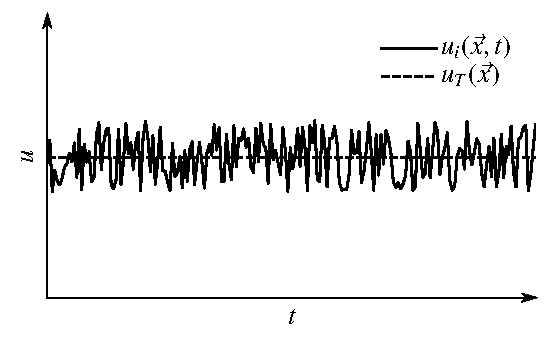
\includegraphics[width=0.7\linewidth]{Pictures/ch7_time_averaging}
	\caption{Time averaging of a stationary flow quantity $u(\vec{x},t).$}
	\label{fig:time_averaging}
\end{figure}
\textit{Homogeneous} flows are those whose properties do not vary in any direction. In this case, a \textit{spatial averaging} procedure may be convenient
\begin{equation}
	u_\Omega(t) = \lim_{\Omega\rightarrow\infty} \frac{1}{\Omega}\int_\Omega u(\vec{x},t)dV,
\end{equation}
where $\Omega$ is the volume of the domain. Finally, \textit{ensemble averaging} can be used to obtain mean values using $N$ identical experiments, even if initial and boundary conditions include infinitesimal perturbations. In this type of averaging, the variation on both the spatial and temporal coordinates is maintained. For $N$ experiments, where $N$ is large, we can calculate
\begin{equation}
	u_N(\vec{x},t) = \lim_{N\rightarrow\infty} \frac{1}{N} \sum_{i=1}^N u_i(\vec{x},t),
\end{equation}
where $u_i({\vec{x},t})$ is the result obtained in the $i$-th experiment. An example of ensemble averaging, can be seen in Figure~\ref{fig:ensemble_averaging} for non-stationary flows, where we discover a smooth sinusoidal behaviour after $N$ experiments have been performed. 

\begin{figure}[htbp]
	\centering
	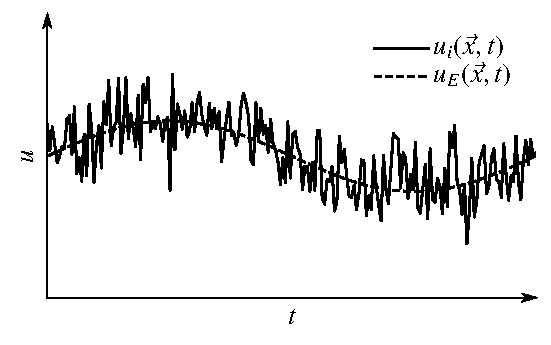
\includegraphics[width=0.7\linewidth]{Pictures/ch7_ensemble_averaging}
	\caption{Ensemble averaging results of a non-stationary flow quantity $u(\vec{x},t).$}
	\label{fig:ensemble_averaging}
\end{figure}

In the following section, we will derive the Reynolds Averaged Navier-Stokes equations using the time-averaging operation. Before we dive into the derivation, we will discuss some Reynolds Averaging properties. For a complete explanation of these properties, refer to Wilcox~\cite{}. 

\subsubsection{Properties of Reynolds Averaging}

Consider a statistically-steady state flow scenario, two flow quantities $u$ and $v$, and constants $\alpha$ and $\beta$.

\begin{itemize}
\item Since the time-averaging process deals with definite integrals, it is a linear operation. Hence, 
\begin{equation}
	\overline{\alpha u + \beta v} = \alpha \overline{u} + \beta \overline{v}.
	\label{eq:reynolds_sum}
\end{equation}
\item The time averaging of integrals and derivatives commute
\begin{equation}
	\overline{\int u dy} = \int \overline{u} dy,  ~~~ \overline{\frac{\partial u}{\partial t}} = \frac{\partial \overline{u}}{\partial t}.
	\label{eq:reynolds_commute}
\end{equation}
\item Any time-averaged fluctuation vanishes, i.e. 
\begin{equation}
	\overline{u^\prime}=0.
	\label{eq:reynolds_fluct}
\end{equation}
\item We can take the average of the product of two instantaneous quantities by
\begin{equation}
	\overline{uv} = \overline{\bar{u}\bar{v}} + \overline{u^\prime v^\prime}.
	\label{eq:reynolds_prod}
\end{equation}
\item From the aforementioned properties, it can also be shown that
\begin{equation}
	\overline{\overline{u}} = \overline{u}, ~~~ \overline{u^\prime \overline{v}} = 0.
	\label{eq:reynolds_avgfluct}
\end{equation}
\end{itemize}

\subsection{The Reynolds Averaged Navier-Stokes Equations}

The Reynolds-Averaged Navier-Stokes (RANS) equations are especially useful for analysis of time-marching numerical methods involving statistically steady flow problems. These equations have been widely used in the aerospace industry for decades. The idea is to split each of the flow variables into mean and fluctuating components and then perform time averaging of the equations. As a consequence, the high-frequency information is removed from the flow. The resulting conservation laws describe only the evolution of the mean flow quantities. 

In this section, we will derive RANS equations for incompressible flow and later for the compressible case. We will then discuss the appearance of the Reynolds stresses as a consequence of time-averaging nonlinear convective terms from the Navier-Stokes equations.

\subsubsection{Incompressible flow}

Consider the incompressible mass conservation law
\begin{equation}
    \nabla\cdot\vec{v} = 0,
\end{equation}
which we rewrite using tensor notation
\begin{equation}
    \frac{\partial v_i}{\partial x_i} = 0,
\end{equation}
where index $i$ indicates summation over all considered directions. We decompose the velocity variable as the sum of mean and fluctuation components
\begin{equation}
    \overline{\frac{\partial }{\partial x_i}\left(\overline{v_i} + v_i^\prime\right)} = 0.
\end{equation}
Since the time-averaging procedure commutes with derivative operators (Equation~\ref{eq:reynolds_commute}),
\begin{equation}
    \label{eq:rans_mass_decomposed}
    \frac{\partial}{\partial x_i} \overline{\left(\overline{v_i} + v_i^\prime\right)} = 0.
\end{equation}
Using Equations~\ref{eq:reynolds_sum} and~\ref{eq:reynolds_fluct},
\begin{eqBox}
\begin{equation}
	\frac{\partial \overline{v_i}}{\partial x_i} = 0,
	\label{eq:rans_continuity}
\end{equation}
\end{eqBox}
where the fluctuating term has vanished. This means that the divergence of each of the terms in Equation~\ref{eq:rans_mass_decomposed} must equal zero. Hence
\begin{equation}
	\frac{\partial v_i^\prime}{\partial x_i} = 0.
	\label{eq:rans_continuity2}
\end{equation}
Next, we consider the momentum equation. Similarly, we split the variables using Reynolds decomposition and then time-average both sides of the equation. The momentum equations can be written using tensor notation
\begin{equation}
    \label{eq:rans_momentum_initial}
    \rho\frac{\partial v_i}{\partial t} + \rho v_j\frac{\partial v_i}{\partial x_j} =
    - \frac{\partial p}{\partial x_i} + \mu \frac{\partial^2 v_i}{\partial x_j^2},
\end{equation}
where $\mu$ is the dynamic viscosity and $\rho=\overline{\rho}$ is constant due to the incompressible condition. We will simplify the derivation beforehand by considering
\begin{equation}
    \frac{\partial \left(v_jv_i\right)}{\partial x_j} = v_j \frac{\partial v_i}{\partial x_j} + v_i \frac{\partial v_j}{\partial x_j},
\end{equation}
where the second term $\partial v_j/\partial x_j$ vanishes according to continuity. Hence,
\begin{equation}
    \frac{\partial \left(v_jv_i\right)}{\partial x_j} = v_j \frac{\partial v_i}{\partial x_j},
\end{equation}
which we use to replace the convective term in Equation~\ref{eq:rans_momentum_initial}, such that
\begin{equation}
    \rho\frac{\partial  v_i}{\partial t} + \rho\frac{\partial  v_j v_i}{\partial x_j} =
    - \frac{\partial p}{\partial x_i} + \mu \frac{\partial^2 v_i}{\partial x_j^2}.
\end{equation}
Decomposing the flow variables and time-averaging the resulting equation, we have
\begin{equation}
    \overline{ 
    \rho\frac{\partial  \left(\overline{v_i}+v_i^\prime\right)}{\partial t} 
    + \rho \frac{\partial  \left(\overline{v_j} + v_j^\prime\right)\left(\overline{v_i}+ v_i^\prime\right)}{\partial x_j}} = \overline{
     - \frac{\partial \left(\overline{p}+p^\prime\right)}{\partial x_i} 
    + \mu \frac{\partial^2 \left(\overline{v_i}
    +v_i^\prime\right)}{\partial x_j^2}}.
\end{equation}
By first resolving multiplications and then applying the Reynolds averaging properties, we obtain the momentum RANS equations for incompressible flow
\begin{eqBox}
\begin{equation}
    \rho \frac{\partial \overline{v_i}}{\partial t} 
    + \rho  \frac{\partial}{\partial x_j} \left(\overline{v_j}\overline{v_i} + \overline{v_j^\prime v_i^\prime}\right)
    =- \frac{\partial \overline{p}}{\partial x_i} 
    + \mu \frac{\partial^2 \overline{v_i}}{\partial x_j^2}.
\end{equation}
\end{eqBox}
Recall the stress tensor $\tau_{ij}$ from Chapter 4, which we now rewrite in tensor notation
\begin{equation}
    \tau_{ij} = 2\mu s_{ij},
\end{equation}
where $s_{ij}$ is the strain-rate tensor
\begin{equation}
    s_{ij} = \frac{1}{2}\left(\frac{\partial v_i}{\partial x_j}+\frac{\partial v_j
    }{\partial x_i}\right).
\end{equation}
We may now rewrite the RANS momentum equation in terms of the stresses and rearrange some terms, such that
\begin{eqBox}
\begin{equation}
    \rho \frac{\partial \overline{v_i}}{\partial t} 
    + \rho  \frac{\partial}{\partial x_j} \left(\overline{v_j}\overline{v_i}\right)
    =- \frac{\partial \overline{p}}{\partial x_i} 
    + \frac{\partial}{\partial x_j} \left(\overline\tau_{ji} - \rho \overline{v_j^\prime v_i^\prime}\right),
\end{equation}
\end{eqBox}
where $\rho \overline{v_j^\prime v_i^\prime}$ is known as the \textit{Reynolds stress}, which we can define as the \textit{Reynolds stress tensor} $\rho\hat\tau_{ij}$, such that
\begin{equation}
	\hat\tau_{ij} = -\overline{v_i^\prime v_j^\prime}.
\end{equation}
It is clear that $\hat\tau_{ij}=\hat\tau_{ji}$, so the Reynolds stress tensor is symmetric. This means that three diagonal components and three off-diagonal components make a total of six independent variables. This number of unknown rises to ten if we consider the properties of three-dimensional flow, i.e. density and the three velocity components ($\rho, \vec{v}$). Clearly, we have an underdetermined system and require additional equations. Later in this chapter, we derive an equation for the Reynolds stresses and discuss some of the consequences that arise from the averaging of the Navier-Stoke equations. We now look at the RANS equations for compressible flow.

\subsubsection{Compressible flow}

In the previous section, we derived the incompressible form of the RANS equations, where the density variations are negligible, i.e $\rho=\overline{\rho}$. In the case of compressible flow, these variations must be now taken into account. However, the equations can become very lengthy and complicated if the conventional averaging procedure is used. To visualize this, let us decompose the mass conservation law using the conventional Reynolds decomposition
\begin{equation}
    \frac{\partial}{\partial t} \left(\overline{\rho} + \rho^\prime\right) + \frac{\partial }{\partial x_i} \left[\left(\overline{\rho}+\rho^\prime\right)\left(\overline{v_i}+v_i^\prime\right)\right] = 0,
\end{equation}
which will introduce correlations involving density fluctuations and may complicate the turbulence modelling, i.e.
\begin{equation}
    \frac{\partial \overline{\rho}}{\partial t}  + \frac{\partial }{\partial x_i} \left(\overline \rho \overline{v_i} + \overline{\rho^\prime v^\prime}\right) = 0.
\end{equation}
By performing a density-weighted time-averaging, introduced by Alexandre Favre in 1969, the equations become simpler and the presence of $\rho^\prime$ can be avoided. It is defined by
\begin{equation}
    \tilde{u}=  \frac{1}{\overline{\rho}} \lim_{n\rightarrow\infty} \frac{1}{n}\sum_{\nu=1}^{\nu=n}\left(\rho u\right)^{(\nu)} = \frac{\overline{\rho u}}{\overline{\rho}},
    \label{eqn:favre_definition}
\end{equation}
where $\overline{\cdot}$ represents the conventional time-averaging. Similar to Reynolds decomposition, we consider the flow properties to be the sum of a mean and fluctuating component
\begin{equation}
    u = \tilde{u} + u^{\prime\prime},
\end{equation}
where $\tilde{u}$ is the \textit{Favre mean} and $u^{\prime\prime}$ is the \textit{Favre fluctuation}. Some properties of the Favre averaging are
\begin{align}
    \overline{\tilde{u}} &= \tilde{u},\\
    \overline{\rho u^{\prime\prime}} &= 0, \\
    \overline{u^{\prime\prime}} &= -\overline{\rho^\prime u^\prime}/{\overline{\rho}}, \\ 
    \overline{\rho u v} &= \overline{\rho}\tilde u\tilde v + \overline{\rho u^{\prime\prime}v^{\prime\prime}}. \label{eqn:favre_rhouv}
\end{align}
We note that $\rho$ is the instantaneous density and that the Favre average differs from the Reynolds averaging properties. For instance, $\overline{u^\prime}=0$, whereas $\overline{u^{\prime\prime}}\neq0$. In addition, the conventional Reynolds and Favre averaging are related by
\begin{align}
    \tilde{u} & = \overline{u} + \overline{\frac{\rho^\prime u^\prime}{\overline \rho}}, \\
    u^{\prime\prime} & = u^\prime - \overline{\frac{\rho^\prime u^\prime}{\overline \rho}}.
\end{align}
We now derive the compressible RANS equations, also known as Favre-Averaged Navier-Stokes Equations (FANS). Starting with conservation of mass, by performing time averaging, we have
\begin{eqBox}
\begin{equation}
    \overline{\frac{\partial\rho}{\partial t}} + \overline{\frac{\partial \rho v_i}{\partial x_i}}= 0.
\end{equation}
\end{eqBox}
Since the time-averaging procedure commutes with the derivatives,
\begin{equation}
    \frac{\partial\overline{\rho}}{\partial t} + \frac{\partial \overline{\rho v_i}}{\partial x_i}= 0.
\end{equation}
The first term can then be Favre decomposed and time averaged
\begin{equation}
    \frac{\partial}{\partial t} \overline{\left(\tilde \rho + \rho^{\prime\prime} \right)} 
    = \frac{\partial \overline \rho}{\partial t},
    \label{eqn:favre_singlevariable}
\end{equation}
and the proof is left as a simple exercise to the reader. The second term $\overline{\rho v_i}$ can be computed using the Favre definition in Equation~\ref{eqn:favre_definition}. The averaged mass conservation equation for compressible flows can then be written
\begin{equation}
    \frac{\partial\overline{\rho}}{\partial t} + \frac{\partial \overline{\rho} \tilde v_i}{\partial x_i}= 0.
\end{equation}
Next, we derive the compressible time-averaged momentum equations. Initially, these are given by 
\begin{equation}
    \frac{\partial }{\partial t} \left(\overline{\rho v_i}\right)
    + \frac{\partial}{\partial x_j} \left(\overline{\rho v_j v_i}\right)
    =- \frac{\partial \overline{p}}{\partial x_i} 
    + \mu \frac{\partial^2 }{\partial x_j^2} \left(\overline{v_i}\right).
\end{equation}
The unsteady term can be computed using Equation~\ref{eqn:favre_definition}. We pay special attention to the convective term, which we expand according to Equation~\ref{eqn:favre_rhouv}
\begin{equation}
    \overline{\rho v_j v_i} = \overline{\rho}\tilde v_j\tilde v_i + \overline{\rho v_j^{\prime\prime} v_i^{\prime\prime}}.
\end{equation}
The time-averaged compressible momentum equations can be written
\begin{eqBox}
\begin{equation}
    \frac{\partial }{\partial t} \left(\overline\rho \tilde v_i \right)
    + \frac{\partial}{\partial x_j} \left(\overline\rho \tilde v_j \tilde v_i + \overline{\rho v_i^{\prime\prime}v_j^{\prime\prime}} \right)
    = - \frac{\partial \overline{p}}{\partial x_i} 
    + \mu \frac{\partial^2 }{\partial x_j^2} \left(\overline{v_i}\right).
\end{equation}
\end{eqBox}
where single-variable terms such as the pressure and diffusive components follow the same procedure described in Equation~\ref{eqn:favre_singlevariable}. Similar to the incompressible case, we rearrange some terms in the equation, such that
\begin{eqBox}
    \begin{equation}
        \frac{\partial }{\partial t} \left(\overline\rho \tilde v_i \right)
        + \frac{\partial}{\partial x_j} \left(\overline\rho \tilde v_j \tilde v_i \right)
        = - \frac{\partial \overline{p}}{\partial x_i} 
        + \mu \frac{\partial }{\partial x_j} \left(\overline{\tau_{ji}} - \overline{\rho v_i^{\prime\prime}v_j^{\prime\prime}}\right).
    \end{equation}
\end{eqBox}
where $-\overline{\rho v_i^{\prime\prime}v_j^{\prime\prime}}$ is the Reynolds stress, which includes the instantaneous density $\rho$, and $\tau_{ij}$ is the viscous stress tensor. As explained in the incompressible section, the resulting system of equations remains underdetermined due to the Reynolds stresses. Obtaining an equation for these stresses turns out to introduce additional unknowns. We now discuss and derive equations for the Reynolds-stress tensor for incompressible flow.

\subsection{The Reynolds Stresses}
As we have previously shown, the Reynolds stresses stem from the averaging of the convective term of the Navier-Stokes equations. We now need to find additional equations to solve our system of time-averaged conservation laws. Specifically, we would like to define equations that describe the rate of change of these stresses as we have done for other flow quantities. In this section, we derive the expressions for incompressible flow, however, the derivation can be readily performed for the compressible case considering the Favre averaging procedure. Hence, consider the incompressible momentum equations in the $i$-th direction, which we conveniently rewrite 
\begin{equation}
	P(v_i) 
	= \rho \frac{\partial v_i}{\partial t}
	+ \rho v_k\frac{\partial v_i}{\partial x_k}
	+ \frac{\partial p}{\partial x_i} 
	- \mu \frac{\partial^2 v_i}{\partial x_k \partial x_k} =0.
\end{equation}
Since we are looking for a time-averaged symmetric tensor for the Reynolds stresses, we perform the following operation
\begin{equation}
	\overline{v_i^\prime P(v_j) + v_j^\prime P(v_i)}=0.
	\label{eq:reynolds_stresses_1}
\end{equation}
Here, $v_i^\prime$ and $v_j^\prime$ are fluctuation components in the $i$-th and $j$-th direction, respectively. We can compactly rewrite Equation~\ref{eq:reynolds_stresses_1} using
\begin{equation}
	A_{ij} + B_{ij} + C_{ij} + D_{ij} = 0,
\end{equation}
where $A_{ij},~B_{ij},~C_{ij},~D_{ij}$ are the unsteady, convective, pressure and viscous stress tensors from the momentum equations, respectively. For the sake of clarity, we expand each of these terms
\begin{align}
	A_{ij} &= \overline{v_i^\prime\rho\frac{\partial v_j}{\partial t} + v_j^\prime\rho\frac{\partial v_i}{\partial t}},\\
	B_{ij} &= \overline{v_i^\prime\rho v_k\frac{\partial v_j}{\partial x_k} + v_j^\prime\rho v_k\frac{\partial v_i}{\partial x_k}},\\
	C_{ij} &= \overline{v_j^\prime\frac{\partial p}{\partial x_i} + v_i^\prime\frac{\partial p}{\partial x_j}}, \\
	D_{ij} &= \overline{-v_i^\prime\mu\frac{\partial^2 v_j}{\partial x_k\partial x_k}-v_j^\prime\mu\frac{\partial^2 v_i}{\partial x_k\partial x_k}}.
\end{align}
We will now time-average and derive an expression for the Reynolds-stress tensor. Initially, we want to split the instantaneous variables using Reynolds decomposition. Starting with the unsteady term
\begin{equation}
	A_{ij}
	=
	\rho\overline{v_i^\prime \frac{\partial}{\partial t}\left(\overline v_j + v_j^\prime \right)} +
	\rho\overline{v_j^\prime \frac{\partial}{\partial t}\left(\overline v_i + v_{i\vphantom{j}}^\prime \right)}, 
\end{equation}
which we rewrite after solving the products
\begin{equation}
	A_{ij}
	=
	\rho \overline{v_i^\prime\frac{\partial\overline v_j^{\vphantom{\prime}}}{\partial t}} 
	+ \rho \overline{v_i^\prime\frac{\partial v_j^\prime}{\partial t}}
	+ \rho \overline{v_j^\prime\frac{\partial\overline v_{i\vphantom{j}}^{\vphantom{\prime}}}{\partial t}} 
	+ \rho \overline{v_j^\prime\frac{\partial v_{i\vphantom{j}}^\prime}{\partial t}}.
	\label{eq:reystress_A_1}
\end{equation}
Recall from the Reynolds averaging properties in Equation~\ref{eq:reynolds_avgfluct} that the average of the product of a mean and a fluctuating quantity is zero. Hence, we eliminate the first and third terms in Equation~\ref{eq:reystress_A_1}. Furthermore, we apply the product rule to bring fluctuation quantities into the temporal derivative. This yields the time-averaged convective term
\begin{eqBox}
\begin{equation}
	A_{ij}
	= \rho \overline{v_i^\prime\frac{\partial v_j^\prime}{\partial t}}
	+ \rho \overline{v_j^\prime\frac{\partial v_{i\vphantom{j}}^\prime}{\partial t}} 
	= \rho \frac{\partial}{\partial t} \left(\overline{v_i^\prime v_j^\prime}\right).
\end{equation}
\end{eqBox}
Next, we decompose the variables in the convective term
\begin{equation}
	B_{ij} =
	\rho \overline{v_i^\prime \left(\overline v_k+v_{k\vphantom{j}}^\prime\right)\frac{\partial}{\partial x_k}\left(\overline v_j+v_j^\prime\right)}
	+ \rho \overline{v_j^\prime \left(\overline v_k+v_{k\vphantom{j}}^\prime\right)\frac{\partial}{\partial x_k}\left(\overline v_i+v_{i\vphantom{j}}^\prime\right)},
\end{equation} 
whereby solving the products, we obtain
\begin{equation}
	\begin{aligned}
	B_{ij} &=
	\overline{v_i^\prime\overline v_k \frac{\partial\overline v_j^{\vphantom{\prime}}}{\partial x_k} }
	+ \overline{v_i^\prime\overline v_k \frac{\partial v_j^\prime}{\partial x_k} }
	+ \overline{v_i^\prime v_k^\prime \frac{\partial\overline v_j^{\vphantom{\prime}}}{\partial x_k} }
	+ \overline{v_i^\prime v_k^\prime \frac{\partial v_j^\prime}{\partial x_k} } \\
	&+ \overline{v_j^\prime\overline v_k \frac{\partial\overline v_i}{\partial x_k} }
	+ \overline{v_j^\prime\overline v_k \frac{\partial v_i^\prime}{\partial x_k} }
	+ \overline{v_j^\prime v_k^\prime \frac{\partial\overline v_i}{\partial x_k} }
	+ \overline{v_j^\prime v_k^\prime \frac{\partial v_i^\prime}{\partial x_k} }.
	\end{aligned}
	\label{eq:reystress_B_1}
\end{equation}
Note that $\overline{u^\prime \overline v \overline w} = \overline{u^\prime} \overline v \overline w = 0$ as a consequence of Equation~\ref{eq:reynolds_avgfluct}. This way we can clean up Equation~\ref{eq:reystress_B_1} by eliminating the first and fifth terms. In addition, using the product rule for the second and fourth term, we have
\begin{equation}
	\overline{v_i^\prime \overline v_k \frac{\partial v_j^\prime}{\partial x_k} }
	+ \overline{v_j^\prime \overline v_k \frac{\partial v_{i\vphantom{j}}^\prime}{\partial x_k} } 
	= \overline v_k \frac{\partial}{\partial x_k} \left(\overline{v_i^\prime v_j^\prime}\right),
\end{equation}
where $\overline v_k$ is a constant. This yields
\begin{equation}
	B_{ij} = \rho \left[\overline v_k \frac{\partial}{\partial x_k} \left(\overline{v_i^\prime v_j^\prime}\right) 
	+ \overline{v_i^\prime v_k^\prime} \frac{\partial\overline v_j}{\partial x_k}
	+ \overline{v_k^\prime \frac{\partial}{\partial x_k} \left(v_i^\prime v_j^\prime\right)}
	+ \overline{v_j^\prime v_k^\prime}\frac{\partial\overline v_{i\vphantom{j}}}{\partial x_k}\right].
	\label{eq:reystress_B_2}
\end{equation}
We can use the chain rule on the third term of Equation~\ref{eq:reystress_B_2}, such that
\begin{equation}
	\frac{\partial}{\partial x_k} \left(\overline{v_i^\prime v_j^\prime v_k^\prime }\right) 
	= \overline{v_i^\prime v_j^\prime \frac{\partial v_k^\prime}{\partial x_k} } 
	+ \overline{v_k^\prime \frac{\partial\vphantom{v_k^\prime}}{\partial x_k}\left(v_i^\prime v_j^\prime\right)} 
	= \overline{v_k^\prime \frac{\partial\vphantom{v_k^\prime}}{\partial x_k}\left(v_i^\prime v_j^\prime\right)},
\end{equation}
where the first term is zero due to continuity (see Equation~\ref{eq:rans_continuity2}). We can now write the time-averaged convective term of the Reynolds stress equation
\begin{eqBox}
\begin{equation}
	B_{ij} = 
	\overline v_k \frac{\partial}{\partial x_k} \left(\rho \overline{v_i^\prime v_j^\prime}\right) 
	+ \rho \overline{v_i^\prime v_k^\prime}\frac{\partial \overline v_j }{\partial x_k}
	+ \frac{\partial}{\partial x_k} \left(\rho \overline{v_i^\prime v_j^\prime v_k^\prime }\right)
	+ \rho \overline{v_j^\prime v_k^\prime}\frac{\partial \overline v_{i\vphantom{j}}}{\partial x_k}.
\end{equation}
\end{eqBox}
Now, we move on to the pressure term. By splitting the instantaneous quantities, we obtain
\begin{equation}
	C_{ij} = 
	\overline{v_i^\prime \frac{\partial}{\partial x_j} \left(\overline p + p^\prime \right)}
	+ \overline{v_j^\prime \frac{\partial}{\partial x_i} \left(\overline p + p^\prime\right)},
\end{equation}
which after solving the products and cancelling the linear terms yields
\begin{eqBox}
\begin{equation}
	C_{ij} =  
	\overline{v_i^\prime \frac{\partial p^\prime}{\partial x_j}}
	+\overline{v_j^\prime \frac{\partial p^\prime}{\partial x_i}}.
\end{equation}
\end{eqBox}
Finally, we decompose the viscous term
\begin{equation}
	D_{ij} = -\mu \left[ 
	  \overline{v_i^\prime \frac{\partial^2}{\partial x_k\partial x_k} \left(\overline v_j + v_j^\prime\right)}
	+ \overline{v_j^\prime \frac{\partial^2}{\partial x_k\partial x_k} \left(\overline v_i + v_{i\vphantom{j}}^\prime\right)}
	\right],
\end{equation}
whereby solving the products and cancelling corresponding terms yields
\begin{equation}
	D_{ij} = -\mu \left[ 
	  \overline{v_i^\prime \frac{\partial^2 v_j^\prime}{\partial x_k\partial x_k}}
	+ \overline{v_j^\prime \frac{\partial^2 v_{i\vphantom{j}}^\prime }{\partial x_k\partial x_k}}
	\right].
\end{equation}
From the chain rule, we can write
\begin{equation}
	\frac{\partial^2}{\partial x_k \partial x_k} \left(\overline{v_i^\prime v_j^\prime} \right) 
	= 2\overline{\frac{\partial v_{i\vphantom{j}}^\prime}{\partial x_k}\frac{\partial v_j^\prime}{\partial x_k}}
	+ \overline{v_i^\prime \frac{\partial^2 v_j^\prime}{\partial x_k\partial x_k}}
	+ \overline{v_j^\prime \frac{\partial^2 v_{i\vphantom{j}}^\prime}{\partial x_k\partial x_k}},
\end{equation}
which yields the time-averaged viscous term
\begin{eqBox}
\begin{equation}
	D_{ij} = -
	\mu \frac{\partial^2}{\partial x_k \partial x_k} \left(\overline{v_i^\prime v_j^\prime}\right) 
	+ 2 \mu \overline{\frac{\partial v_{i\vphantom{j}}^\prime}{\partial x_k}\frac{\partial v_j^\prime}{\partial x_k}}.
\end{equation}
\end{eqBox}
The resulting equation for the evolution of the Reynolds stresses can be written as
\begin{equation}
	\begin{aligned}
	\frac{\partial}{\partial t} \left(\rho \overline{v_i^\prime v_j^\prime}\right) 
	+ \overline v_k \frac{\partial}{\partial x_k} \left(\rho \overline{v_i^\prime v_j^\prime}\right) 
	=&
	- \rho \overline{v_i^\prime v_k^\prime}\frac{\partial \overline v_j }{\partial x_k}
	- \rho \overline{v_j^\prime v_k^\prime}\frac{\partial \overline v_{i\vphantom{j}}}{\partial x_k}
	- \overline{v_i^\prime \frac{\partial p^\prime}{\partial x_j}}
	- \overline{v_j^\prime \frac{\partial p^\prime}{\partial x_i}}  \\
	&+ \frac{\partial^2}{\partial x_k}  
	\left[
		\mu \frac{\partial}{\partial x_k} \left(\overline{v_i^\prime v_j^\prime}\right)
		- \left(\rho\overline{v_i^\prime v_j^\prime v_k^\prime }\right) 
	\right]
	- 2 \mu \overline{\frac{\partial v_{i\vphantom{j}}^\prime}{\partial x_k}\frac{\partial v_j^\prime}{\partial x_k}}.
	\end{aligned}
	\label{eq:reynolds_stress_eq}
\end{equation}
By inspecting Equation~\ref{eq:reynolds_stress_eq}, it is clear that we have added six equations, but the number of unknowns also increased. The high-order correlation $\overline{v_i^\prime v_j^\prime v_k^\prime}$ is responsible for ten additional unknowns, in addition to other twelve that result from the new pressure and viscosity terms. This is known as the \textit{closure} problem of turbulence. Interestingly, if we decided to further find equations by taking additional moments, new higher-order correlations would appear. This is a consequence of the initial averaging of the Navier-Stokes equations. By multiplying Equation~\ref{eq:reynolds_stress_eq} by $-\rho^{-1}$ and using the following definitions
\begin{align}
	\hat\tau_{ij} &= -\overline{v_i^\prime v_j^\prime},\\
	\Pi_{ij} &= \overline{\frac{p^\prime}{\rho} \left(\frac{\partial v_i^\prime}{\partial x_j} + \frac{\partial v_j^\prime}{\partial x_j} \right)}, \\
	\epsilon_{ij} &= 2\nu \overline{\frac{\partial v_i^\prime}{\partial x_k}}\overline{\frac{\partial v_j^\prime}{\partial x_k}},\\
	\rho C_{ijk} &= \rho \overline{v_i^\prime v_j^\prime v_k^\prime} + \overline{p^\prime v_i^\prime}\delta_{jk} + \overline{p^\prime v_j^\prime}\delta_{ik},
\end{align}
we can compactly write the Reynolds-stress equation in its common form
\begin{eqBox}
	\begin{equation}
		\frac{\partial \hat \tau_{ij}}{\partial t} + \overline v_k \frac{\partial \hat \tau_{ij}}{\partial x_k}
		= - \hat\tau_{ij}\frac{\partial \overline v_j}{\partial x_k} 
		- \hat\tau_{jk}\frac{\partial \overline v_i }{\partial x_k} 
		+ \epsilon_{ij} - \Pi_{ij}
		+ \frac{\partial}{\partial x_k} \left(\nu \frac{\partial \hat\tau_{ij}}{\partial x_k} + C_{ijk}\right).
	\end{equation}
\end{eqBox}
We are still left with a system of equations that remains to be closed. In the quest of solving turbulent flows using the RANS equations, we dedicate the rest of this chapter to the derivation of common algebraic models that have been devised to give closure to these equations.
\section{Turbulence Modelling}
\subsection{The Boussinesq Hypothesis}
\subsection{The Mixing Length Model}
\subsection{The Spalart-Allmaras Model}
\subsection{The k-$\epsilon$ Model}
\subsection{The k-$\omega$ Model}
\subsection{Summary of Turbulence Models}

\chapter{Boundary Conditions}
\section{Wall Boundaries}
\subsection{Wall-Bounded Turbulence}
\subsection{Boundary Conditions}
\subsection{Wall Modelling}
\section{Farfield Boundaries}
\subsection{Non-Reflecting Boundaries}